\chapter{Emotions and facial analysis}

%%%%%%%%%%%%%%%%%%%%%%%%%%%%%%%%%%%%%%%%%%%%%%%%%%%%%%%%%%%%%%%%%%%%%%%%%%%%%%%%%%%%%%%%%%%%%%%%%%%%%%%
\section{Face detection techniques}
%%%%%%%%%%%%%%%%%%%%%%%%%%%%%%%%%%%%%%%%%%%%%%%%%%%%%%%%%%%%%%%%%%%%%%%%%%%%%%%%%%%%%%%%%%%%%%%%%%%%%%%
Computer Vision, a subarea of Computer Graphics, is the scientific domain that aims to make computers perceive the world in a similar way that humans do. Computer vision systems usually rely on image processing, artificial intelligence (e.g. machine learning) and decision making techniques to detect and classify objects from images or videos. A class of such objects is human faces, detected and analyzed by a process called facial alignment. Facial alignment consists of identifying the position of specific features of the face, e.g. eye and nose, after the face has been detected in an image/video. Figure \ref{fig:alignment} demonstrates the process.

\begin{figure}[ht]
    \centering
    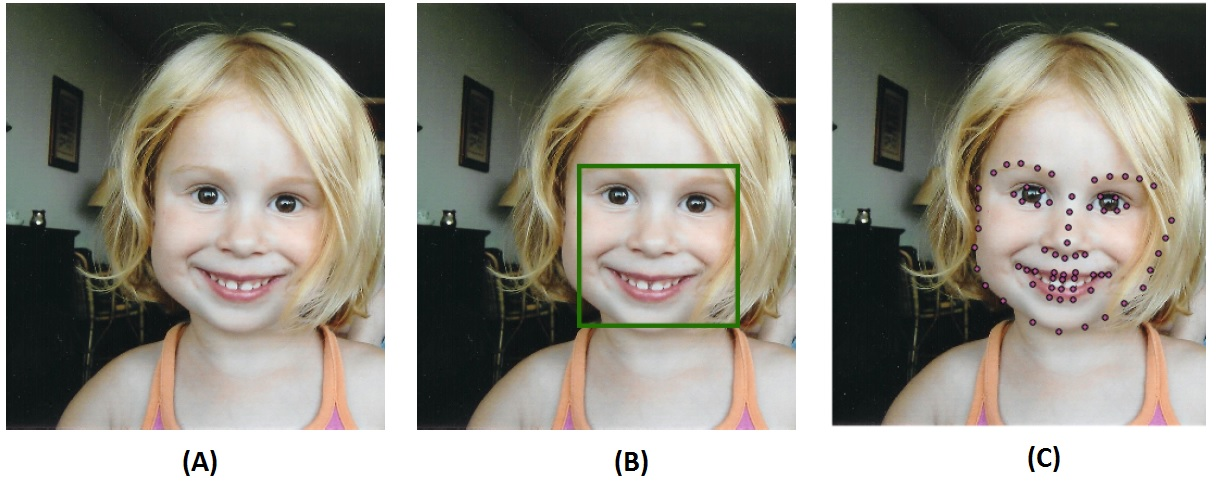
\includegraphics[width=0.8\linewidth]{figures/face_alignment.jpg}
    \caption{Example of face alignment. (A) Input image. (B) Detected face. (C) Aligned face.}
    \label{fig:alignment}
\end{figure}

This procedure is relevant in many different scenarios, for instance facial/expression recognition and pose estimation. Research has been conducted to create accurate and fast methods that can be used to perform face alignment under an ever growing set of challenging conditions, e.g. face movement combined with different lighting configurations. Many methods have been proposed and a literature review shows that two basic approaches are widely used in alignment techniques: constrained local models and cascaded regression methods. Both approaches work on an image of a face contained within a rectangle obtained by a face detection algorithm, such as Viola \& Jones \parencite{viola2004robust}. The following sections describe each one of them, mentioning the most relevant techniques for facial alignment that are based on the approach being described.

\subsection{Constrained Local Model}

The Constrained Local Model (CLM) approach consists of locating a set of points on a target image, then applying a constrain to them. The constrain is usually based on a statistical shape model, which is obtained via training in a set of images featuring manually inserted landmarks. Since the shape model is statistical, the position of the points (landmarks) that it describes will always resemble a face, so proportions of lines and/or the distance among points will not be so different from a human face (at least not different from the ones found in the training set). Figure \ref{fig:clm-model-variation} illustrates the configuration of the shape model with different variations.

\begin{figure}[ht]
    \centering
    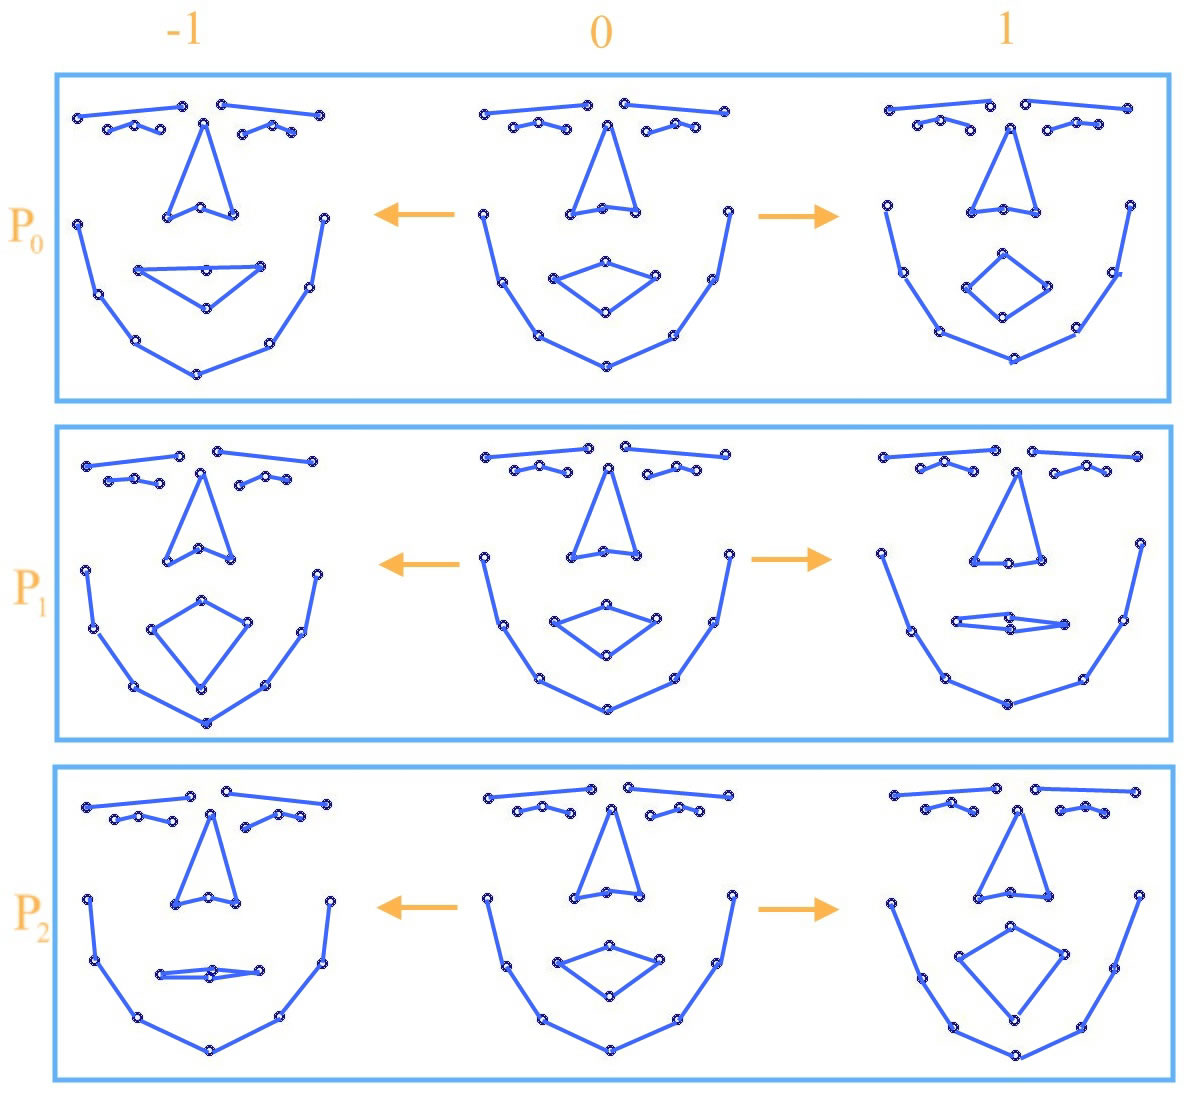
\includegraphics[width=0.6\linewidth]{figures/clm-model-variation.jpg}
    \caption{Configuration of the shape models with different variations \parencite{yu2010facial}.}
    \label{fig:clm-model-variation}
\end{figure}

Additionally to the shape model, there is a texture model that contains a set of patches (images) extracted from the training images by selecting the areas around the inserted landmarks. Those patches are used to guide the search procedure in the alignment process, which allows the technique to correctly identify the right model to properly align the face being analyzed. Figure \ref{fig:clm-patches} shows different shape models and their respective entries in the texture model. The process of aligning a face is iterative and it starts by sampling points that are placed in the face image according to the current shape estimation of the face. In the first try, this estimation is usually the average face obtained from all training images. The area around the sampled points are extracted and used in a search to locate a set of similar patches in the texture model. The current shape estimation and the texture patches it locates are evaluated according to a cost function. As soon as the shape variation with the minimal cost is found, the process is repeated: new patches are sampled and searched against the texture model, the current estimation is adjusted and so on. Eventually the current estimation will sample areas that precisely match very specific patch textures in the model, so the points will converge and they can be used to align the face.

\begin{figure}[ht]
    \centering
    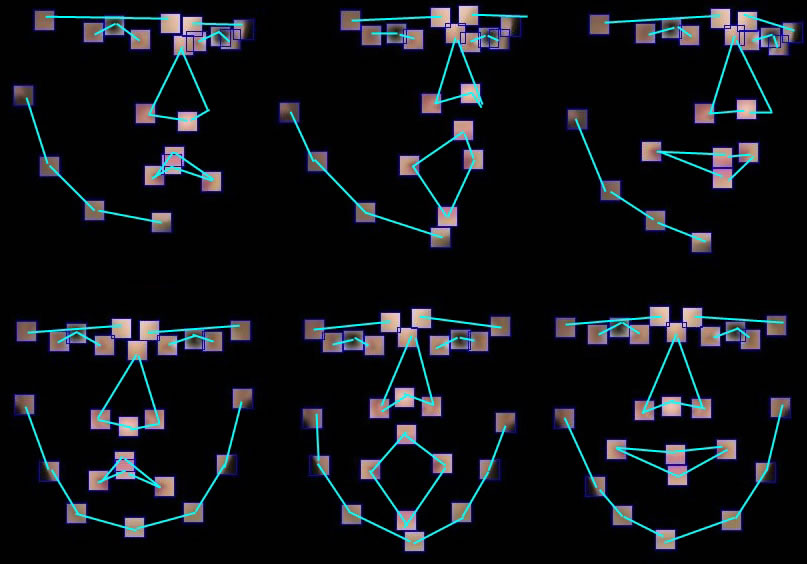
\includegraphics[width=0.6\linewidth]{figures/clm-patches.jpg}
    \caption{Shape models and their respective entries in the texture model \parencite{yu2010facial}.}
    \label{fig:clm-patches}
\end{figure}

Figure \ref{fig:clm-evolution} demonstrates the evolution of the technique as it iterates in an image. In Figure \ref{fig:clm-evolution}-(a), the mean shape is placed into the image and the patches are sampled around the (mistakenly) positioned landmarks. As the technique iterates ((b) and (c)), searched patches progressively induce changes in the current shape model, sampling more accurate patches. Eventually the technique converges to the aligned face, presented in Figure \ref{fig:clm-evolution}-(d).

\begin{figure}[ht]
    \centering
    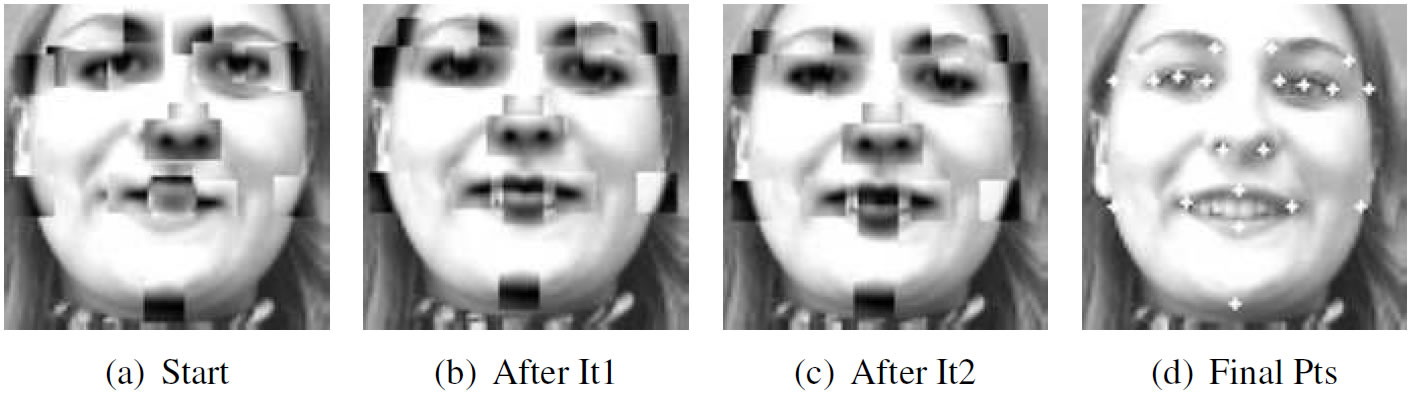
\includegraphics[width=0.9\linewidth]{figures/clm-evolution.jpg}
    \caption{Iteration of CLM during the alignment of an image \parencite{cristinacce2006feature}.}
    \label{fig:clm-evolution}
\end{figure}

Two techniques that represent the CLM approach are the feature detection and tracking with constrained local models \parencite{cristinacce2006feature} and its 3D variation \parencite{baltruvsaitis20123d}, which uses 3D depth data to improve the process.

\subsection{Cascaded Regression}

The cascaded regression methods approach consists of using an initial guess shape that is progressively refined into the final answer (identification of key features in the image). This refinement is performed in a stage-by-stage manner (cascade) and the result of the current stage is used as the input for the next one. In each stage, the adjustment of the current shape (into the aligned result) is performed by a regression function, learnt via training. Early regressors in the cascade handle large variations in the shape, as opposed to the late ones, which focus on specific details. Each regressor extracts features from the image, which are then worked to produce variations in the current guess shape. The extracted features depend on the current shape and they are commonly referred as shape-indexed features.

The shape-indexed features are differences in pixel intensities. The calculation of a shape-indexed feature involves the selection of a few pixels and the subtraction of their intensities. The way those pixels are selected is usually different for each of the cascaded-regression techniques. Figure \ref{fig:shape-indexed} illustrates an example of selection of a few pixels for three particular landmarks; the landmark on the top-right (gray circle) highlights the selected pixels that will be used. The difference of intensities among those pixels will define this particular shape-indexed local feature. The shape-indexed local features are used in a decision process in each step (cascade), as illustrated by Figure \ref{fig:regressor-steps}. Usually the initial guess shape is the mean shape of the training set. This guess is used to calculate the current set of shape-indexed features to be extracted, which then guides the variation applied to the current shape. The variation to be applied is usually chosen based on the result of a cost function, which selects a variation that minimizes the distance between the current guess and the supposed aligned face. As the process repeats itself, different shape-indexed features are selected, a new variation is calculated and so on. Eventually the current shape will converge and it will represent the alignment for the face being analyzed (final shape estimation).

\begin{figure}[ht]
    \centering
    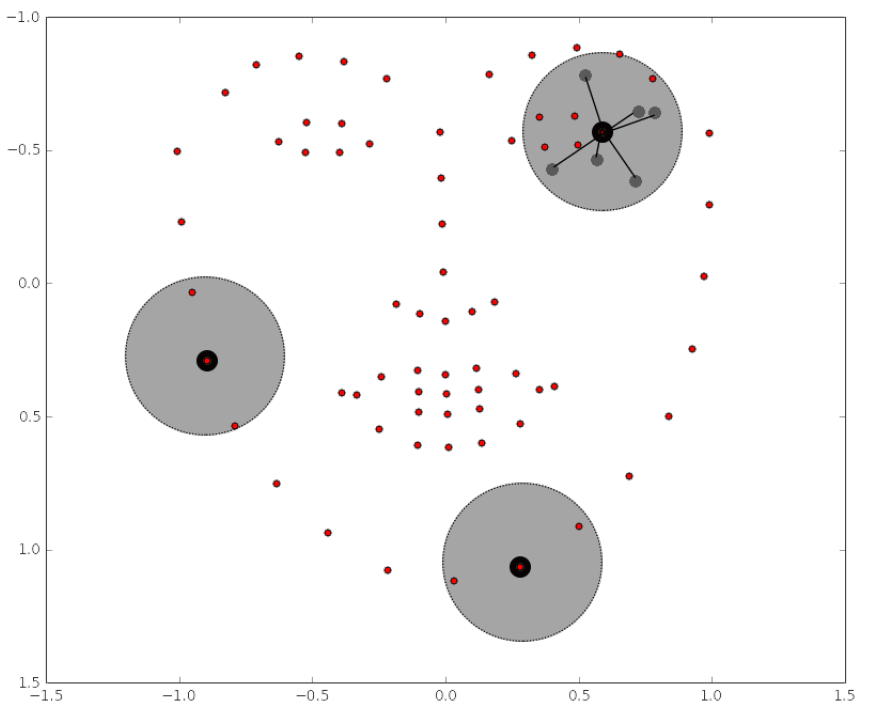
\includegraphics[width=0.7\linewidth]{figures/shape-indexed.png}
    \caption{Pixels used in the calculation of a shape-indexed feature \parencite{maris2015}.}
    \label{fig:shape-indexed}
\end{figure}

\begin{figure}[ht]
    \centering
    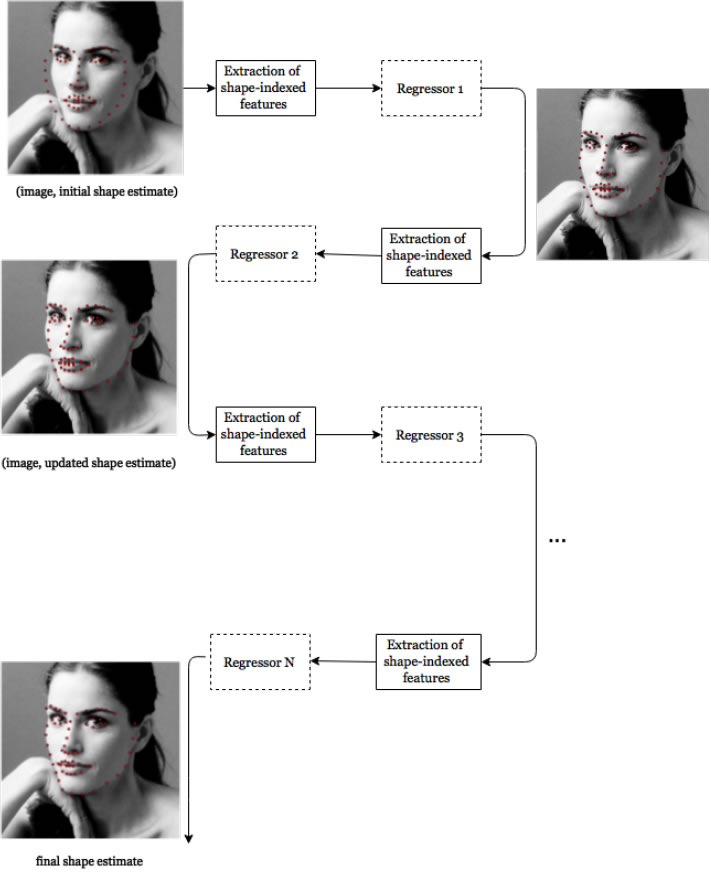
\includegraphics[width=0.9\linewidth]{figures/cascade-explanation.jpg}
    \caption{Estimation of face shape with regressors in a set of stages \parencite{maris2015}.}
    \label{fig:regressor-steps}
\end{figure}

Different variations are used to handle the training, the extraction of features and the way the regression is performed. The technique of face alignment with Ensemble of Regression Trees (ERT) \parencite{kazemi2014one}, for instance, estimates the face's landmarks by inputting the regressors with a sparse subset of pixels intensities, which is calculated with a prior probability on the distance of the pixels. The Supervised Descent Method (SDM) \parencite{xiong2013supervised}, on the other hand, extracts SIFT features from the current shape estimation and it converges the shape by solving a series of linear least square problems. The approach via regression of Local Binary Features (LBF) \parencite{ren2014face} proposes the use of a set of local binary features (opposed to a global view of the face) combined with a locality principle for learning and processing such features independently. Finally the face alignment by Explicit Shape Regression (ESR) \parencite{cao2014face} trains the regressors by explicitly minimizing the alignment error over training data, so all facial landmarks are regressed jointly. The regressors work by progressively inferring the shape, so the early regressors in the cascade handle large shape variations (ensures robustness) while later regressors focus on the small and subtle variations (ensures accuracy).

%%%%%%%%%%%%%%%%%%%%%%%%%%%%%%%%%%%%%%%%%%%%%%%%%%%%%%%%%%%%%%%%%%%%%%%%%%%%%%%%%%%%%%%%%%%%%%%%%%%%%%%
\section{Facial features and emotion detection}
%%%%%%%%%%%%%%%%%%%%%%%%%%%%%%%%%%%%%%%%%%%%%%%%%%%%%%%%%%%%%%%%%%%%%%%%%%%%%%%%%%%%%%%%%%%%%%%%%%%%%%%



%%%%%%%%%%%%%%%%%%%%%%%%%%%%%%%%%%%%%%%%%%%%%%%%%%%%%%%%%%%%%%%%%%%%%%%%%%%%%%%%%%%%%%%%%%%%%%%%%%%%%%%
\section{Emotion detection based on facial movement}
%%%%%%%%%%%%%%%%%%%%%%%%%%%%%%%%%%%%%%%%%%%%%%%%%%%%%%%%%%%%%%%%%%%%%%%%%%%%%%%%%%%%%%%%%%%%%%%%%%%%%%%
